%!TEX root = ../main.tex
\documentclass[a4paper,oneside,12pt, class=Latex/Classes/PhDthesisPSnPDF, crop=false]{standalone}
\usepackage{setspace}
\begin{document}
\doublespacing
\chapter{Observing in the optical regime}
\label{chap:obs}

\color{red}To do list: Add refs, run by NOT for sanity check, get consistent with \ztfg\ vs \ztfg$\arcmin$ (ask at NOT), sometimes slightly confused which tense to use, recheck carefully, opmaak, reference about the LP light pollution restriction laws? mention gain (e$^-$ / ADU conversion) and read noise (mean e$^-$ added per pixel at readout) as well somewhere. \color{black}

Astrophysicists face the challenge of not being able to set up and control their experiments. The universe is our laboratory but all we can do is see or detect the results while often not knowing the exact setup of the experiment. Models are made to explain and predict the behaviour of planets, stars, galaxies, etc. but ultimately observations are needed to compare against and test our models. My work relies heavily on observational data, and in this chapter I will introduce the different types of observations that are used throughout this thesis (section~\ref{observation_types}), telescopes and instruments that are used to obtain these observations (section~\ref{telescopes}), and a quick overview of how to calibrate the raw images and extract useful data (sections~\ref{calibration} and~\ref{reduction}). I will also give a general overview of what to consider when planning observations in section~\ref{considerations}.


\section{Types of obeservations}
\label{observation_types}{}
All optical observations are, in esssence, images taken by a camera. Light falls onto a pixel on the detector, a charge-coupled-device (CCD), and frees some amount of electrons. The more light that hits the pixel, the more electrons are freed. At readout these electrons are counted per pixel, or group of pixels if binning is applied, and turned into a digital number called a count. During this process there are contributions from different noise sources, but as long as the total count rate is in the linear regime of the CCD there is a linear relation between the received flux and final count. It is then possible to calculate the observed flux from the target by using calibration images. The different types of calibration images are described in section~\ref{calibration} and their usage is explained in section~\ref{reduction} when discussing image reduction.


\subsection{Photometry}
\begin{figure}
    \centering
    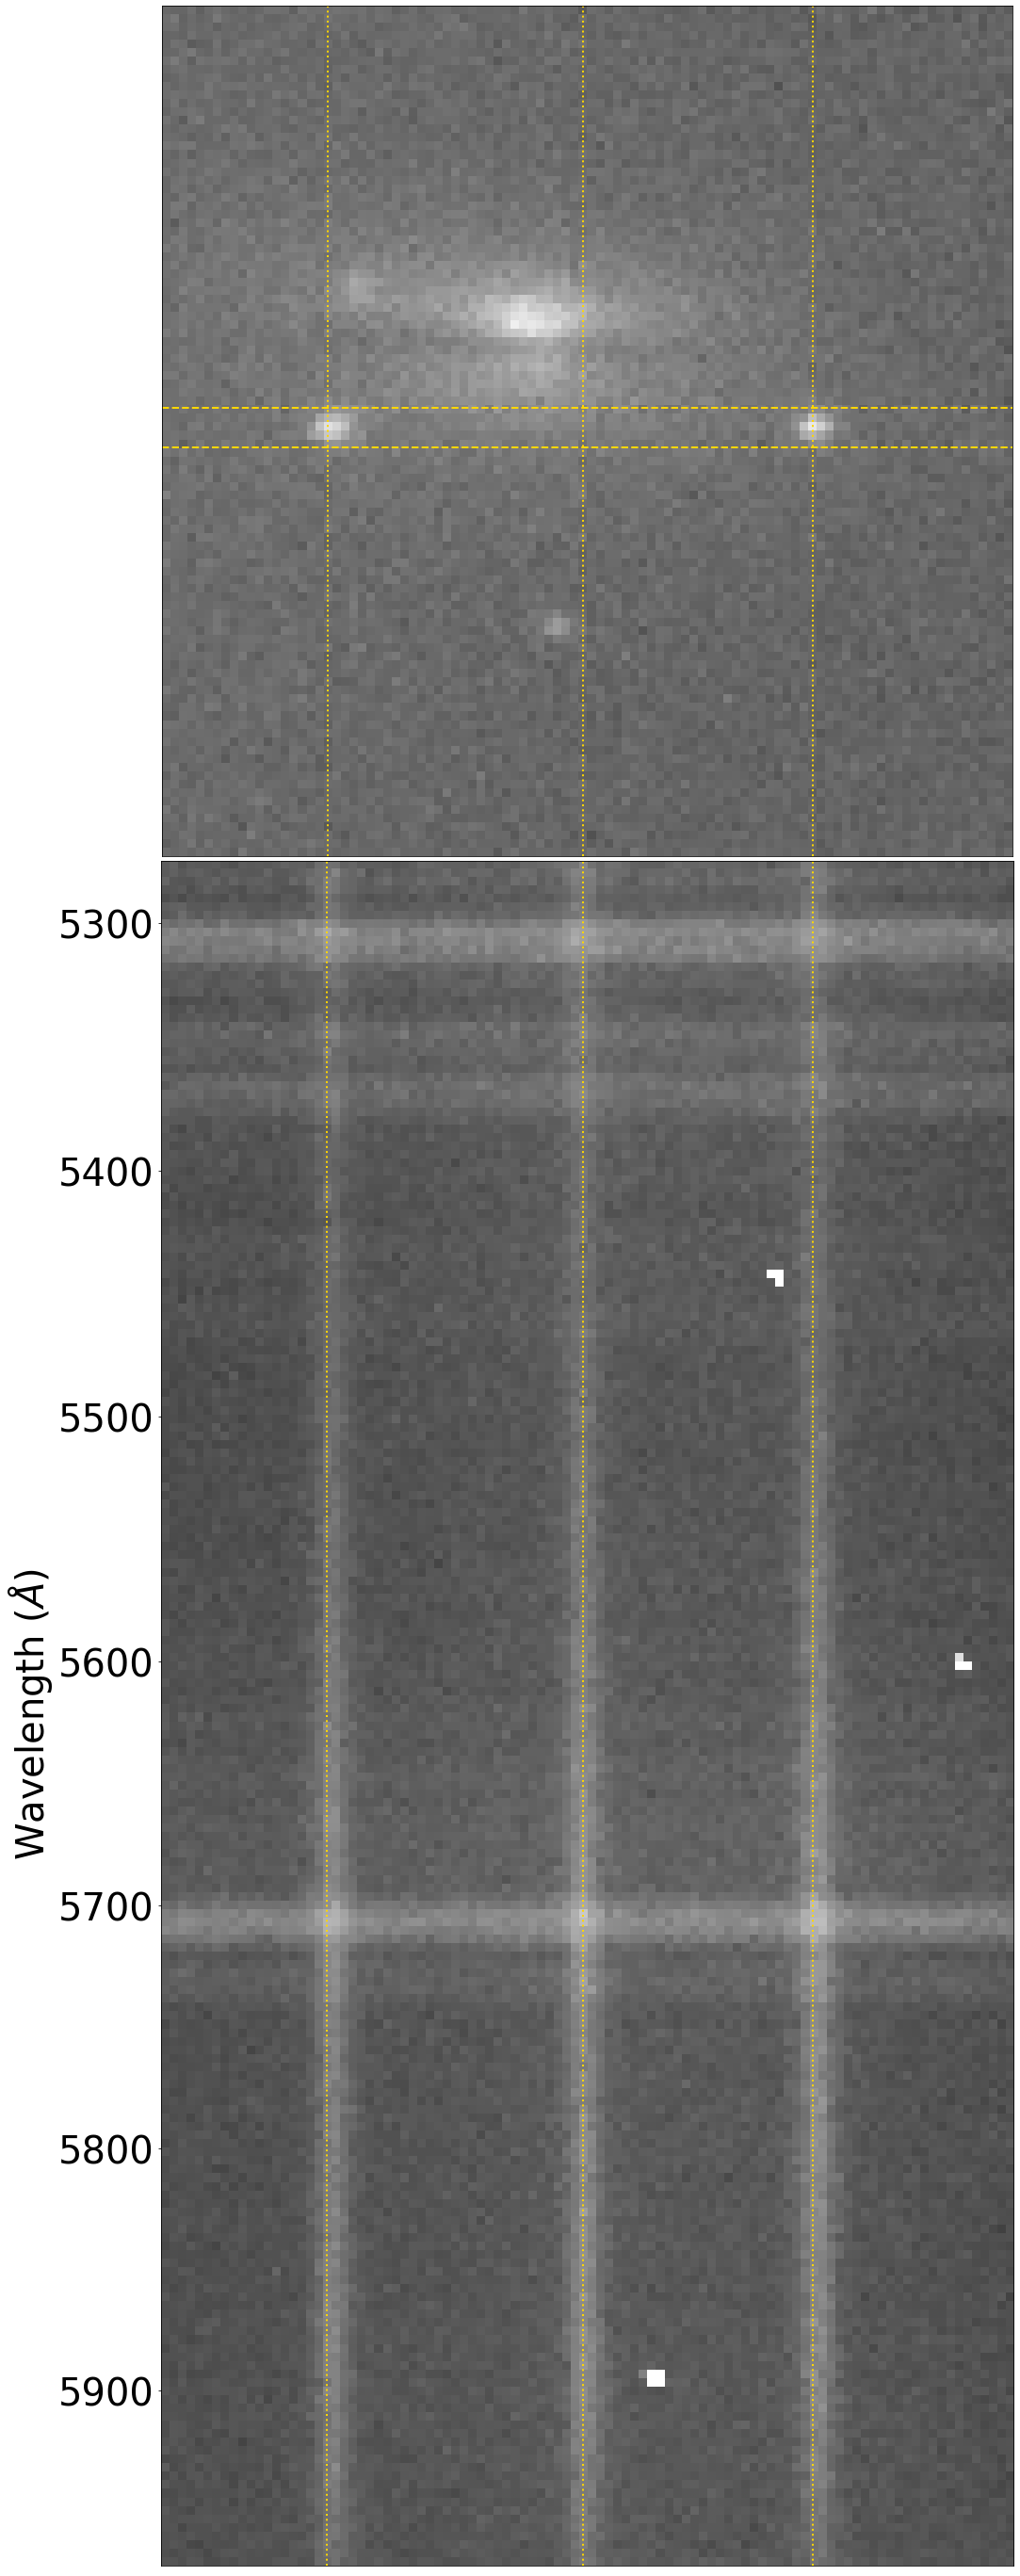
\includegraphics[height=0.8\textheight]{../Images/chapter_2/phot_and_spec_example.png}
    \caption{Image and partial spectrum of SN~2024nqr (left) and SN~2024pgd (right), two SNe Ia active simultaniously in the same galaxy. The image was taken without a filter and used to align the 1.0$\arcsec$ slit (horizontal dashed lines) over both SNe. The resulting spectrum, taken with grism \#4, shows three traces as white vertical stripes. The outer two line up with the two SNe, while the middle trace is from the host galaxy edge in the slit (vertical dotted lines for guidance). The horizontal lines in the spectrum are sky lines coming from atmospheric emission, and the white spots in the spectrum are due to cosmic rays. This data was taken with NOT/ALFOSC on the night of 28 July 2024 while testing an experimental rapid response mode (RRM, credit: Samuel Grund S\o rensen). \color{red}check AT/SN status weirdness \color{black}}
    \label{phot_spec_example}
\end{figure}


Photometry is one of the simplest observing modes as it is just taking a photo of a part of the sky. The top of Fig.~\ref{phot_spec_example} shows a raw photometric image, taken with ALFOSC on the Nordic Optical Telescope (NOT) without the use of a filter. The images are monochromatic, i.e. they only have a value for the intensity. For colourful images multiple observations have to be made using different filters and combined to represent different colours. Faint objects can be observed by increasing the exposure time in a single image, or by stacking multiple images together to increase the effective exposure time. Stacking images can be useful for e.g. reducing cosmic ray interference, avoiding overexposure of a bright source close to a fainter target, or for constructing time series. When stacking images it is common practice to dither the telescope: applying a small offset between exposures to ensure that the target hits a different part of the CCD to avoid issues with bad pixels ruining otherwise good observations. While this decreases the effective size of the fully stacked image, as long as the edges are not needed there is no issue.

\subsection{Spectroscopy}
Spectroscopy goes one step beyond just taking a photo. Assuming that this is slit spectroscopy, instead of a filter to select a wavelength range to observe now a slit restricts the observable region of the sky to a narrow band along one axis of the detector (e.g. horizontal). After the slit the light hits a grating or grism (a grating and prism combined) which diffracts the light based on wavelength across the second axis of the detector (vertical). The rule density on the grating / grism dictates the wavelength spread of the light: the more rules per unit distance, the bigger the diffraction, and the higher the spectral resolution of the resulting image. The tradeoff is that a smaller part of the spectrum can be observed at a time, and there is less light being received per pixel which reduces the SNR unless the exposure time is increased to account for this. Any point-like source that is observed becomes a line in the spectral direction, called a trace. Extended sources create extended traces.

There is some freedom in the orientation of the slit. This is called the position angle of the slit. If there are multiple targets near each other, and they can be in the slit at the same time, the required position angle can be calculated from the two target positions. If there is a single target to be observed the position angle can be anything, but usually the parallactic angle is chosen. In this orientation the slit is perpendicular to the horizon, and prevents losses from differential diffraction (different colours diffracting differently when entering the atmosphere at an angle, \citealt{diff_refrac_atmosphere}). The trace will only be slightly diagonal on the CCD.

The bottom panel of Fig.~\ref{phot_spec_example} shows a section of the spectrum taken of the SNe in the top panel image. The two SNe are drawn out into vertical traces and a third trace belonging to the edge of the host galaxy can be seen in the middle. The horizontal lines are sky emission lines, and while these can technically be used to estimate the conversion from pixel position to wavelength, standardized arc frames will result in a much better wavelength calibration (see section~\ref{reduction}).


\section{Telescopes}
\label{telescopes}
Most of the data used in this thesis comes from the Zwicky Transient Facility (ZTF), and follow-up observations have been made using the Nordic Optical Telescope (NOT), and the Gran Telescopio Canarias (GTC), which will be introduced below. Some additional data comes from other sources, which are listed for completeness. The same filter names (\ztfg\ztfr\ztfi) are used for filters at different telescopes,  which have slight differences. In the rest of this thesis I will use \ztfg\ztfr\ztfi to refer to the ZTF filters, unless specified otherwise. \color{red} gotta make sure this is done correctly everywhere \color{black}

\subsection{Zwicky Transient Facility}
The Zwicky Transient Facility (ZTF, \citealt{ZTF_Surveys_Scheduler, ZTF_overview_and_1st_results, ZTF_Science_Objectives, ZTF_Instrumentation, ZTF_Observing_System}) is an optical large-sky survey observing the entire northern night sky above Dec $\approx -30$\degree\ every 2 to 3 nights in three broadband optical filters \ztfg~($\lambda_{eff} = 4746.48$ \AA), \ztfr~($\lambda_{eff} = 6366.38$ \AA), and \ztfi~($\lambda_{eff} = 7829.03$ \AA), which are similar to the well-known SDSS \ztfg\ztfr\ztfi\ filters. The efficiency of these filters is plotted as a function of wavelength in Fig. \ref{Optical_elements_plot}. The survey saw first light in October 2017 and the survey formally began scientific operation in March 2018, and has been running continueously until the time of writing this document.

The observations are made using the $48\arcsec$ aperture Schmidt-type design Samuel Oschin Telescope, which is based at the Palomar Observatory in Southern California. Each exposure is 30 s long, can go a limiting magnitude of $\sim20.5$ mag and covers an area of $\sim47$ deg$^2$ at a resolution of of $1.01\arcsec$ per pixel. The camera is divided in a $4\times4$ grid of CCDs, each of which have 4 readout channels called quadrants. This results in each observation producing 64 separate images, each with their own readout channel identifier (rcid). Similarly, the observed region of the sky is divided into different telescope pointings called fields to ensure that the same region of the sky is observed in the same way each time, aiding with the reduction of the data. This results in each combination of filter, field, and rcid being a set of observations of a particular part of the sky using specific setup.

\begin{figure}
    \centering
    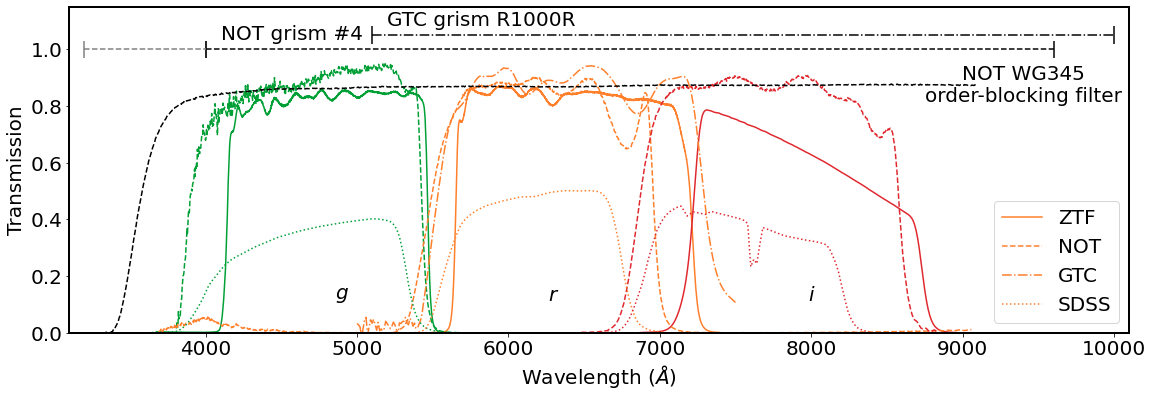
\includegraphics[width=\textwidth]{../Images/chapter_2/transmissions.png}
    \caption{Throughput as a function of wavelength of the different filters used to gather the bulk of the data in this thesis \ztfg filters are shown in green, \ztfr in orange, \ztfi in red, and the different telescopes are shown with different line styles (Continuous for ZTF, dashed for NOT, dot-dashed for GTC). The SDSS filters (dotted lines) are shown for comparison. For the grisms the wavelength ranges are shown as only, not their efficiency at each wavelength.}
    \label{Optical_elements_plot}
\end{figure}


\subsection{Nordic Optical Telescope}
The Nordic Optical Telescope (NOT \footnote{\url{https://not.iac.es}}) is a 2.56 m telescope located at Observatorio Roque de Los Muchacos in La Palma, Spain, at an elevation of 2382 m above sea level. It hosts several instruments for observing in the optical and near infrared, both for imaging and spectroscopy. The Alhambra Faint Object Spectrograph and Camera (ALFOSC) was used to obtain the data used in this thesis. I will only discuss the parts relevant to this thesis, further details on this instrument and  details on the other instruments can be found at the NOT website.

ALFOSC is a versatile instrument mounted in cassegrain and can be used for imaging, spectroscopy, and (spectro)polarimtery. As there are several wheels equipped to hold a variety of optical elements, the instrument can switch quickly between different setups between observations. The images can cover up to $6.4\arcmin\times6.4\arcmin$ per exposure at a resolution of $0.2138\arcsec$ per pixel. In this thesis \ztfg~($\lambda_{cen} = 4800$ \AA), \ztfr~($\lambda_{cen} = 6180$ \AA), and \ztfi~($\lambda_{cen} = 7710$ \AA) are used for photometry. For spectroscopy grism \#4 is used to split the light vertically, together with a horizontal $1.0\arcsec$ slit if the seeing was $\leq1.3\arcsec$ or a horizontal $1.3\arcsec$ slit if the seeing was $\geq1.3\arcsec$. Grism \#4 has a resolution of 3.3 \AA\ pixel$^{-1}$ and an wavelength range from 3200 \AA\ to 9600 \AA, but as the response at short wavelengths is poor, the spectra used in this thesis are cut at 4000 \AA. For some spectra an order-blocking filter (WG345) is used as well to avoid second order diffracted blue light to overlap with first order diffracted red light on the detector. The transmission curves of the filters and wavelength range of the grism are shown in Fig.~\ref{Optical_elements_plot}.
%Details on these optical elements are given in Table \ref{NOT_optic_elems}, and they are shown in Fig. \ref{Optical_elements_plot}.

\begin{comment}
\begin{table}
    \centering
    \caption{Optical elements used for observations taken with NOT/ALFOSC and GTC/OSIRIS+. \color{red} Check the $\arcmin$ symbols necessity and make sure to stay consistent \color{black}}
    %\resizebox{\textwidth}{!}{%Scale table to page width
    	\begin{tabular}{ccccc}
    		\hline
    		\hline
    		Filter & $\lambda_\text{center}$ (\AA) & FWHM (\AA) & T$_\text{max}$\\
    		\hline
    		\ztfg$\arcmin$ NOT & 4800 & 1450 & 0.92\\
    		\ztfr$\arcmin$ NOT & 6180 & 1480 & 0.90\\
    		\ztfr$\arcmin$ GTC & 6410 & 1760 & 0.94\\
    		\ztfi$\arcmin$ NOT & 7710 & 1710 & 0.91\\
    		WG345 & 3560 & - & 0.88\\
    		\\
    		\hline
    		\hline
    		Grism & $\lambda$ range (\AA) & resolution (\AA / pixel) & Orientation\\
    		\hline
    		\#4 & 3200$^*$ - 9600 & 3.3 & vertical\\
    		R1000R & 5100 - 10000 & 2.62 & horizontal\\
    		\\
    		\hline
    		\hline
    		slit & Telescope & Orientation\\
    		\hline
    		1.0$\arcsec$ & NOT & horizontal & \\
    		1.0$\arcsec$ & GTC & vertical & \\
    		1.3$\arcsec$ & NOT & horizontal & \\
    		\hline
    	\end{tabular}
    %}
    \begin{flushleft}
    	$^*$ The detector response is limited at low wavelengths, so in practice a lower limit of 4000 \AA\ is used for the spectra in this thesis.
    \end{flushleft}
    \label{NOT_optic_elems}
\end{table}
\end{comment}

\subsection{Gran Telescopio CANARIAS}
The Gran Telescopio CANARIAS (GTC \footnote{\url{https://www.gtc.iac.es}}) is a 10.4 m telescope at Observatorio Roque de los Muchachos in La Palma, Spain, and is the largest optical / near infrared telescope on the island. Its primary mirror is made up from 36 hexagonal pieces creating an effective collection area of 73 m$^2$, ideal for observing very faint targets. The GTC can host up to six instruments at a time in various focal positions, allowing for a large variety of observations to be made. One of the most commonly used instruments is OSIRIS+, the upgraded version of OSIRIS: the Optical System for Imaging and low-Intermediate-Resolution Integrated Spectroscopy.

OSIRIS+ has an unvignetted field-of-view of $7.8\arcmin\times7.8\arcmin$ at a resolution of $0.254\arcsec$ per pixel. Since the standard readout has $2\times2$ binning, the resolution can be increased to $0.127\arcsec$ per pixel if so desired. Like ALFOSC, this instrument is also built to easily switch between different setups between observations. For photometry the \ztfr ($\lambda_{cen} =6410$ \AA) filter is used in this thesis, and for spectroscopy the R1000R grism with a $1.0\arcsec$ vertical slit is used. R1000R splits the light horizontally over the detector with a range of 5100 \AA to 10000 \AA\ with a resolution of 2.62 \AA\ pixel$^{-1}$ These filter transmission curve and grism wavelength range are shown in Fig.~\ref{Optical_elements_plot}.
%Details on the optical elements are given in Table \ref{NOT_optic_elems}, and they are shown in Fig. \ref{Optical_elements_plot}.% ' after the filter?


\subsection{Other observations}
Small amounts of data coming from other telescopes and surveys are presented in this thesis as well. This includes a follow-up observation of SN~2019ldf in section \color{red} PUT REFERENCE ONCE SECTION IS IN \color{black} in \ztfg\ and \ztfr\ using the ESO Faint Object Spectrograph and Camera version 2 (EFOSC2, \citealt{EFOSC2}) imaging spectrograph on the ESO New Technology Telescope (NTT) in La Silla, Chile as part of the extended Public ESO Spectroscopic Survey of Transient Objects+ (EPESSTO+, \citealt{PESSTO}).

To complement ZTF data of several SNe, in chapters \color{red} PUT REFERENCES ONES SECTIONS ARE IN, MIGHT BE DIFFICULT TO DO SECTION SPECIFIC FOR THIS \color{black} optical photometry from the Panoramic Survey Telescope and Rapid Response System (Pan-STARRS, \citealt{Pan-STARRS1}), (intermediate) Palomar Transient Factory (PTF, \citealt{PTF_1, PTF_2}, iPTF, \citealt{iPTF}), All Sky Automated Survey for SuperNovae (ASASSN, \citealt{ASASSN_paper1, ASASSN_catalog}), Asteroid Terrestrial-impact Last Alert System (ATLAS, \citealt{ATLAS}),  and Global Astrometric Interferometer for Astrophysics (Gaia, \citealt{Gaia}) are used, as well as near-infrared photometry from the Wide-Field Infrared Survey Explorer (WISE, \citealt{WISE}).


\section{Calibration images}
\label{calibration}
Before the observations can be used for science, the images need to be calibrated. This is done using different types of calibration images, each of which measure and correct for different effects of the telescope and detector. Usually these are taken during the day or twilight so no valuable observing time is lost. It is standard practice to take multiple calibration images and use an odd number in the reduction to find median values and remove interference from e.g. cosmic rays, this is called a master image.


\subsection{Bias}
The first type of calibration image is the bias, which is made by reading out the CCD without exposing. The resulting image contains the amount of counts that will be in every exposure regardless of what has been observed or with what exposure time. In other words, measuring the bias can be tought of as measuring the offset to correct for in every other image.

%$B_{ij}$ is the so-called bias, the measured pixel response that is in every observation regardless of the exposure time and amount of light hitting the pixel. The easiest way to measure this value is to take bias frames: observe with an exposure time of 0 with no light hitting the CCD. $F$ and $t$ are 0 which reduces Eq.~\ref{CCD_response} to $R_{ij}(0, 0) = B_{ij}$

\subsection{Dark}
Any detector that is not at a temperature of 0 K will have some amount of noise due to thermal effects. This can free electrons in pixels over time, creating a dark current and increasing the noise over time. The effect can be measured by exposing for the same amount of time as the science images taken, but without letting any light hit the CCD. This is called a dark frame.

As this is a thermal effect, it can be reduced to negligible amounts by cooling the instrument. This saves precious observing time, as otherwise dark frames would ideally have to be taken at the same temperature as the target was observed, which is easiest to do directly after the science exposure. By cooling the detector with e.g. liquid nitrogen this noise source can be avoided instead of having to correct for, saving time and the amount of images that need to be taken in the process.

%Next is $D_{ij}$, the noise that increases with longer exposure times. This is thermal noise, and as its name suggests it is more impactful the higher the temperature $T$ is in the CCD: $D_{ij} = D_{ij}(T)$. Due to this there are actually two ways to remove this source of noise. One can take Dark frames by exposing for some amount of time but making sure no light hits the detector, $R_{ij}(0, t) = B_{ij} + D_{ij} \times t$, and extract $D_{ij}$. This takes however a lot of time, and it is often more efficient to cool the CCD down to very low temperatures (e.g. with liquid nitrogen) to ensure $D_{ij}$ can be neglected.

\subsection{Flatfield}
The amount of light that the telescope receives is converted into a digital number, but there is no guarantee that this conversion rate is the same for each pixel. This can be due to intrinsic differences between the pixels, or outside effects such as dust reducing the amount of light recieved on a part of the detector. To correct for this an evenly illuminated field has to be observed, resulting in an image called a flat or flatfield. By ensuring that each pixel receives the same amount of light, the different counts will reflect the varying responses per pixel.

Any evenly illuminated object can be used for this, such as the the inside of the telescope dome to create dome flats. A more perfect evenly lit source however is the sky, and using this sky flats can be taken. While it is usually too bright during the day and the CCD will saturate even with the narrowest filter and shortest exposure time, there is a window during twilight where the sky is darker but not dark enough to observe stars yet, perfect for taking flats. As a general rule, narrowband filters need a brighter sky and in the evening these need to be done before the broadband filters. After that, assuming similar efficiencies between filters, blue filters need brighter skies than red filters, forcing a specific order in which the sky flats need to be taken during the short window where this is possible. Of course if flats are taken in the morning the order has to be reversed.

%Lastly, to measure $A_{ij}$ flatfield images are needed. During a science exposure the amount of light hitting a pixel is dependent of the brightness of the source at that location, $F = F_{ij}$. But as not every pixel may have the same response the measured values need to be normalized before different pixels can be compared. This is done by observing an evenly lit background where $F_{ij}$ is the same for every pixel. This can be done by observing the inside of the dome (dome flats), although the twilight sky (sky flats) are usually preferred as they are more evenly lit across the CCD.

\subsection{Arc}
In spectroscopy one of the axes has low wavelength at one end and high wavelength at the other end of the image. To know where each wavelength falls on the detector, arc frames are needed. These are taken by observing a lamp filled with a known set of elements (e.g. He, Ne, or TH and Ar). The wavelengths of the emission lines are known very precisely, and by matching these with the observed lines in the arc image a pixel-to-wavelength conversion can be found, called the wavelength solution.

Usually arcs can be taken during the day, when the telescope is idle. However in some cases the mechanical flexure of the telescope, caused by being in a different position during observing, can introduce an uncertainty in the wavelength calibration unless an arc is taken with the telescope in the same position as for the target. In these cases an arc is usually taken directly before or after the target is observed, or between exposures of the target.

%For spectroscopy another type of calibration is needed: Wavelength calibration. This is done with arc frames: observing the known emission lines of several elements using lamps in the instrument (e.g. He, Ne, ThAr lamps) using the same setup as the science observation. The resulting pattern of emission lines is known and can be used to map the pixel position in the spectral direction to a wavelength, called the wavelength solution.

\section{Reduction}
\label{reduction}
After all observations have been taken it is time to analyze them. The first step is to reduce the raw data into the required format to work with. After that, additional analysis technique can manipulate the reduced images directly or the data that has been extracted from them. The response function of a detector can be written as

\begin{equation}
	R_{ij}(f, t, \lambda) = B_{ij} + D_{ij}(t) + F_{ij}(\lambda) \times f \times t,
	\label{CCD_response}
\end{equation}

where $R_{ij}$ is the CCD response of pixel $i,j$ as a function of the integrated flux of the target $f \times t$ during the exposure which lasted a time $t$. The goal is to measure the flux $f$, which requires knowing and correcting for the bias level $B_{ij}$, dark current $D_{ij}$, and pixel response $F_{ij}$. Each type of calibration image is used to measure one of these values. Note that it is assumed that there are no cross or higher order terms in Eq.~\ref{CCD_response}, in other words, the CCD is in its linear regime. When a pixel receives too much light and gets close to saturation it is no longer in its linear regime, and more terms appear in Eq.~\ref{CCD_response} making it much more difficult or even impossible to measure the observed flux.


\subsection{Bias, dark, and flat corrections}
Using the calibration images from section~\ref{calibration}, the raw science images can be reduced to something a flux level can be measured from. 

First the master-bias is created and subtracted from every other image. As both $F$ and $t$ are 0, the bias measures $B_{ij}$ directly and can then immediately be removed.

With the bias gone, the dark frames measure $D_{ij}$ for a specific $t$, but the master-dark can only be used on sciene observations with the same exposure time. Alternatively it is possible to subtract $B_{ij} + D_{ij}(t)$ in a single step by not separating out the bias term using bias images first.

Finally every science image is divided through the normalized master-flat to equalize the pixel responses. There is still a factor $F(\lambda)$ present as the detector efficiency is wavelength dependent, but the value is now indepentent of the pixel position, allowing values from across the CCD to be compared.

\subsection{Cosmic-ray removal and image stacking}
At this point it is often good practice to run a cosmic-ray removal algorith to remove this source of noise as much as possible. This can be done using e.g. L.A.Cosmic \citep{lacosmic}, which I used through Astro-SCRAPPY \citep{astroSCRAPPY} when reducing follow-up photometry of several objects in this thesis.

If multiple images are taken of the same field or object they can be stacked to reduce background noise and increase the SNR of the observed objects. Sometimes the observations have been taken with dithering to avoid the same objects being on the same pixels in every exposure, which has to be taken care of to make sure that the images are stacked correctly.

\subsection{Standard star calibration}
Filters are never 100\% transparent at any wavelength, and the CCD responds differently to different wavelengths as well. To correct for this, one last type of calibration image is used: the standard star. This was not mentioned in section~\ref{observation_types} as observing a standard star is exactly the same as observing the actual science target. The only difference is that the expected result of the observation is known and can be used to correct for the wavelength depent efficiency of the instrument.

With photometry the observed brightness can be measured for each star in the image to get a list of instrument magnitudes. The relative differences between the magnitudes of objects are correct, but there is still an absolute offset across all objects. This is corrected by finding the offset using the standard star. If the filter is commonly used, there is a good chance many stars in the field have known magnitudes in that filter, which can be used for calibration instead of a dedicated standard star.

In spectroscopy the arcs are used to find the wavelength solution for the spectra, after which the trace from the standard star can be extracted and divided by the known spectrum of the star to obtain the sensitivity function of the detector $F(\lambda)$. The trace of the target can be extracted as well to get its spectrum, which can then be flux-calibrated using the sensitivity function. In some cases only a relative sensitivity function is known, resulting in a calibrated spectrum in an unknown flux unit. In these cases proper calibrated photometry of the obect can be used to flux-calibrate the spectrum by integrating the spectrum over the filter transmission curve.


\begin{comment} %USE IMAGE ELSEWHERE?
\subsection{Difference imaging}
Transients are, by definition, objects that appear on the sky for a limited amount of time. A popular and effective way to search for new objects is difference imaging. If there is a map or image of how a part of the sky looked some time ago, it can be used as a reference and subtracted from an image of the current sky. Constant sources such as most stars and galaxies (except variable ones) can be removed. To computers images are nothing more than big matrices. This means that, if properly aligned, subtracting the reference from the science images is an easy operation that leaves only those sources whose brightness has changed between the two observations in the so-called difference image. This also ensures that only the transient light is measured in cases where different sources are superimposed, such as a SN superimposed on top of its host galaxy. Figure~\ref{diff_im_example} shows an example of the resulting difference image after subtracting the reference image from the science image.

\begin{figure}
    \centering
    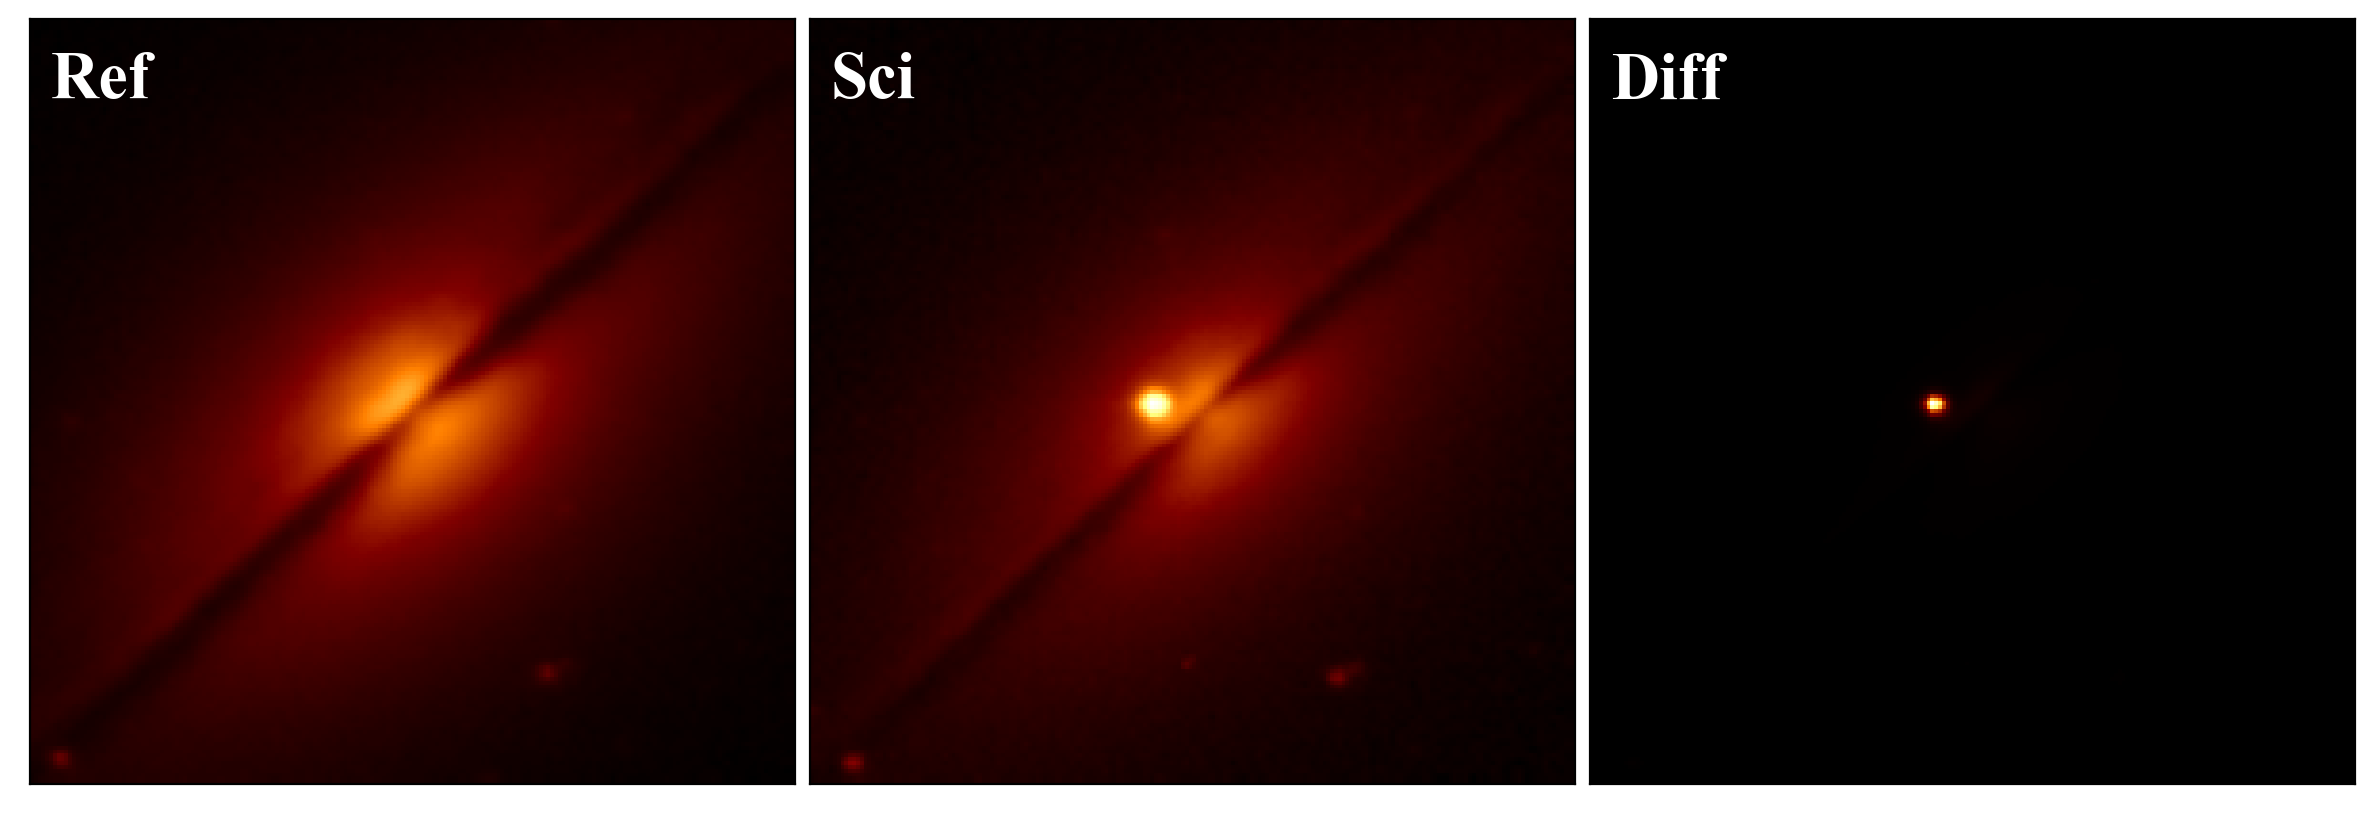
\includegraphics[width=\textwidth]{../Images/chapter_2/diff_im_SN2021rhu.png}
    \caption{Example of a \ztfr-band reference image of NGC 7814, the science image of the same region, and the resulting difference image with the host galaxy removed and only the transient (SN~2021rhu, SN Ia 86G-like) remaining. Credit: Luke Harvey}
    \label{diff_im_example}
\end{figure}
\end{comment}

\subsection{Forced photometry}
The two most common methods to measure flux from as source in an photometric image are PSF photometry and aperture photometry. A good explanation of these can be found in \citet{Photometry_techniques}. PSF stands for point spread function, and with this method a function is fitted to model the source. This function describes how an infinitely small point of light is spread over the detector, and through its spatial size and peak value the flux of the light source can be measured. Aperture photometry sums up the signal in a given radius around the source center and subtracts the contribution from the background in the same region.

%\color{red} See \url{https://coolwiki.ipac.caltech.edu/index.php/Aperture_Photometry_Overview} for references \color{black}

Large surveys such as ZTF observe the night sky to find new transients and monitor known ones. Difference imaging is used to subtract constant sources and reveal active transients, as these are the main sources that should be left in the difference image. Through PSF photometry the location and strength of each source in the image is determined, which are then compared to the locations of known sources to separate new from known ones. Each location has however been observed for the entire duration of the survey, which means that it is also possible to measure the flux of a known transient before and after it was visible in the images, creating a light curve for the full duration of the survey.

This is called forced photometry, because the PSF function is forced to center on a specific location instead of finding the best-fitting position for the centroid. When there is nothing but noise at that location the measured flux will be 0 within the error. When there is a source at the target location it will be measured, but if the source is not at the center of the PSF the fit will have trouble converging, resulting in a large uncertainty. Artefacts such as cosmic rays, imperfectly subtracted difference images, or light bleeding effects from saturated bright nearby stars can also affect the accuracy of the photometry measurement. \color{red} Not completely happy with talking about difference imaging without really introducing it, introduce it here so can keep it bit higher level, mention ZOGY, HOTPANTS, Autophot \color{black}

%\section{The SuperNova Animation Program}
%The light curve that is the result of applying forced photometry at a specific location for the entire run of a survey can contain bad data points. Many of these will be flagged for having a bad PSF fit, bad weather conditions, etc. But even after filtering these out it can be helpful to check the difference images themselves for unexpected behavouir that might be captured in the light curve. For this I created the SuperNova Animation Program (\textsc{snap} \footnote{\url{https://github.com/JTerwel/SuperNova_Animation_Program}})

%\textsc{snap} collects image cutouts of the specified location during the  specified time period(s) and in the specified filter(s). It then matches these with the individual data points in the light curve and puts the images in an animation in chronological order with the reference images at the start. This enables easy identification of bad points due to image defects, off-center sources, residual from imperfectly subtracted sources, cosmic rays etc.

%\section{Simulations}
%Some experiments are difficult or even impossible to do multiple times, one cannot rerun a survey to observe the same transient events. So to understand the biases in the data as well as the effective size of the survey, it needs to be simulated. I used \textsc{simsurvey} \citep{simsurvey,simsurvey_main} \footnote{\url{https://github.com/ZwickyTransientFacility/simsurvey/tree/master}} to simulate an observing campaign like ZTF detecting a specific event under different circumstances. For \textsc{simsurvey} to work both the observer and observed have to be specified, i.e. a model of the telescope, observatory, and survey is required, as well as a model of the transient and where to place it. More details on how the simulation is run are given in section \color{red}ref to paper 1 sim section \color{black}


\section{General considerations for observing}
\label{considerations}
During my PhD I have spent two years doing studentships at the Isaac Newton Group of Telescopes (ING) and Nordic Optical Telescope (NOT) on La Palma, gaining first-hand experience with the specifics of observing in the optical regime and the considerations that come with it. I will briefly go over these in this section.

%To observe astronomical objects one has to consider several things. Assuming that the location or region on the sky to target is already known, as well as what type of data to collect, an observing plan can be made. A well constructed observing plan should allow to obtain the best quality data possible while making efficient use of the resources available.


\subsection{Location}
Although this is normally already done before constructing a telescope, the first thing to consider is the observing location. When purely aiming for the best observations possible, there are three main things to consider when choosing where to observe from:
\begin{itemize}
    \item {Weather: Clear, stable sky conditions for most nights of the year, and low atmospheric distortion (e.g. seeing) are vital to ensure good quality data on a regular basis. Low hanging clouds can be avoided by being high above sea level, while simultaneously decreasing the amount of air light has to travel through to reach the detector, decreasing atmospheric influence.}
    \item {Light pollution: Darker skies allow observations of fainter objects. Even the the presence of a (partially) illuminated moon significantly changes the depth that can be reached with the same exposure time. Many observatories have (inter)national laws to control the ligth pollution and ensure good quality data can be obtained.}
    \item {Target observability: The target location needs to be reachable by the telescope to be observable. The closer to zenith an observation is made, the less atmosphere between the target and telescope. The atmosphere reduces the data quality through turbulence (seeing), broadband absorbtion (clouds, dust), narrowband interference (tellurics, skylines), and differential diffraction, among others.}
\end{itemize}

Observatories should be located on top of high mountains in areas with stable and clear weather, with as small a nearby population as possible while still being accessible enough for transporting materials and observing staff. One of the best locations in the world that meets these requirements is Roque de los Muchachos on La Palma, a small Spanish island in the Atlantic ocean off the coast of Morocco. At around 2300 m above sea level, the telescopes are built on the highest peak of the mountain far from most communities on the island which are much closer to sea level, and the temperate climate ensures good sky conditions for most nights around the year. Additionally, the government has put laws in place to minimize light pollution, e.g. by limiting the use of street lights and restricting flight paths over the island. \color{red} I remember a plaque at the roque mentioning this, maybe it has a good ref? \color{black}


\subsection{Telescope, instrument, observation type, and setup}
Depending on the type of observations and the brightness of the target there is a choice of hardware to be used. Telescope, intsrument, observation type, and desired setup(s) have to be considered together, as some choices will affect other ones.

Bigger telescopes can observe fainter targets, but it is also more difficult to obtain observing time. On the other hand, smaller telescopes are less oversubscribed (a measure of requested versus available observing time), but are more limited in observation depth even with long exposure times. %Small telescopes are however ideal for bright targets that would instantly saturate the detector of a larger telescope if no filter was used.

Secondly, different instruments, which are often telescope specific, have different observing capabilities. Photometry and spectroscopy are very standard observing modes, and most telescopes have at least one instrument can offer this. Even though ALFOSC and OSIRIS+ can both of these modes, there are still differences in data quality and resolution even if the same object is observed at the same time. However for polarimetric observations for instance, OSIRIS+ cannot be used while ALFOSC can, limiting the options for this observation mode.

Lastly, the specific setup has to be considered as well. For photometry, which filters are desired? If a very specific or rare filter is needed this may limit the options of telescopes and instruments. For spectrocopy there are other choices, such as fiber or slit spectroscopy, different gratings or grisms depending on the desired resolution and wavelength range, neutral density filters to observe targets that are otherwise too bright for the instrument, and order-blocking filters to remove second order blue light from red parts of the spectrum.


\subsection{Night plan}
Lastly, it is good to have a plan of what to observe at each point during the night in order to avoid losing observing time during the night. Most proposals already have a list of targets and standard stars to observe and exposure times when they are submitted to request observation time, but the detailed plan is usually made mere hours before the night starts as it depends on e.g. the current weather, target priority, and specific time constraints (e.g. for transits). Calibration images might need to be taken during the night as well. All of these things need to be concidered when trying to maximize the time used to expose and observe targets, and minimize the overheads from e.g. positioning, target acquisition, and readout.

Time spent repositioning the telescope can be reduced by finding the path between targets that minimizes telescope and dome movement throughout the night. The target acquisition time depends on the type of observation, but also on the experience and tiredness of the observer. With photometry a field is observed, so usually a small offset is not disastrous for the science. With spectroscopy the target needs to be identified and placed in the slit or fiber before the exposure can start, costing extra time. Readout times are detector specific, but can be sped up by windowing and binning if only a part of the CCD is needed, and a worse resolution is acceptable. Considering readout times can be especially important when multiple shorter exposures are taken instead of a single long one.

Nothing is certain during the night. Weather conditions can change suddenly, technical problems can occur, a high priority target can be discovered during the night, or observations might go so smoothly that they are completed faster than expected. A flexible schedule with a priority list and backup targets helps adapting to these situations quickly. After all, an idling telescope in (half-)decent observing conditions is a waste of resources. Fig.~\ref{visplot} shows an example night plan for the NOT with some space for adaptibility built in.

\begin{figure}
    \centering
    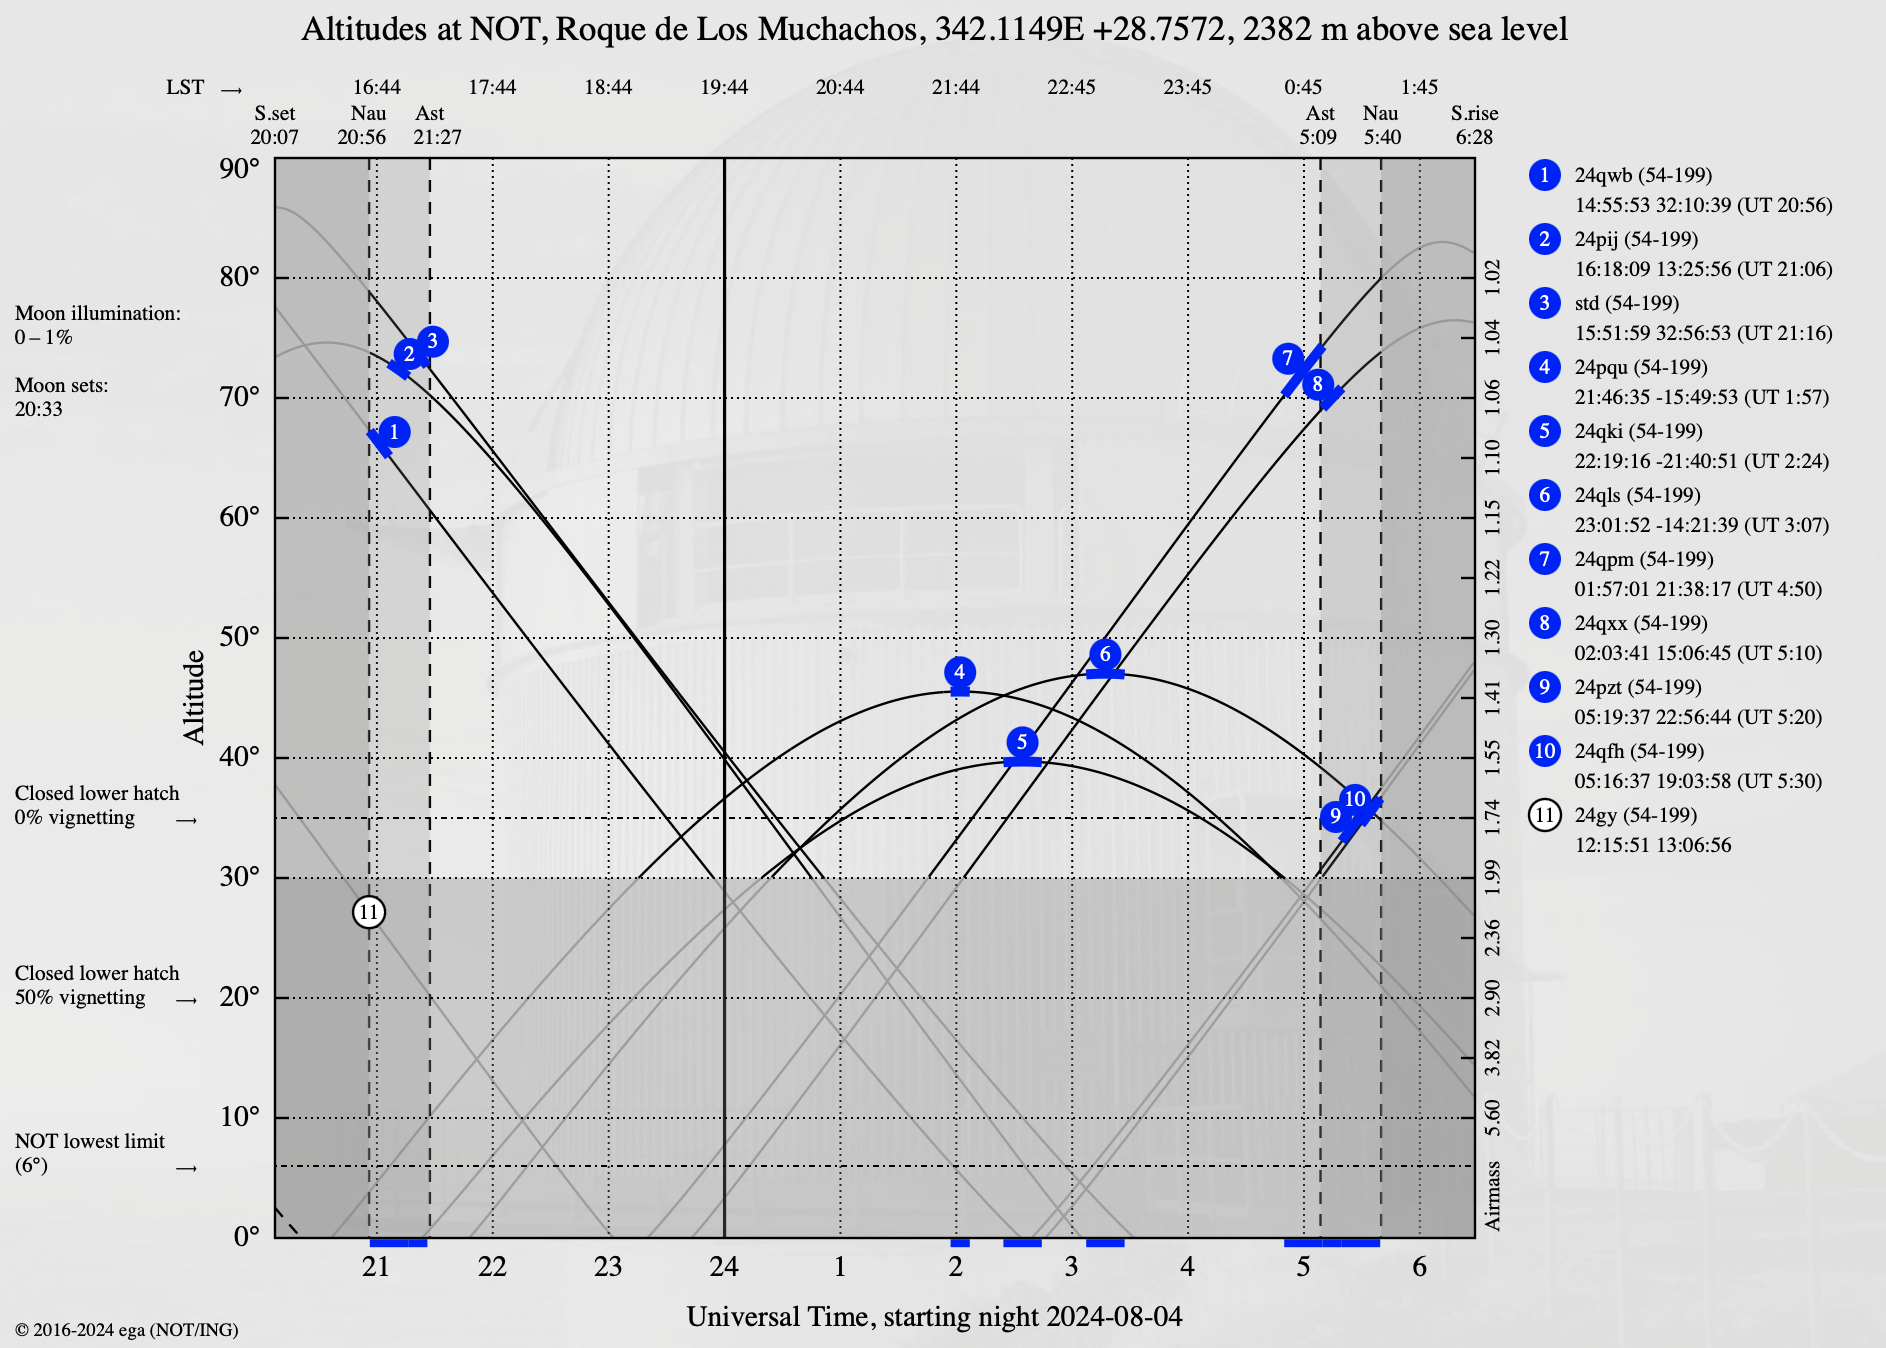
\includegraphics[width=0.95\textwidth]{../Images/chapter_2/visplot.png}
    \caption{Night plan for the NOT on the night of 10 August 2024. Targets are plotted with their altidute as a function of universal standard time. Local stellar time is shown on top. The target priority has been colour coded, with the coloured bars showing the amount of time each observation is expected to take. Green targets have already been completed, and the red vertical line shows the current time. Several unscheduled backup targets are shown in case the plan has to be updated during the night.}
    \label{visplot}
\end{figure}



\end{document}